\chapter{Review of Literature}

Since the autonomy idea starts to grow in the robotic field, 
there are numerous works are presented in the literature for 
different localization techniques with different approaches 
in sensor configuration, data fusion methodologies, connectivity 
and feature map creation. In this chapter, different type of sensors
and different approaches are investigated in order to draw boundary of 
the thesis and to get the better vision about the robot localization.

\section{Sensors in Mobile Robotics}
In this section, sensors which are used for solving localization problem is studied in sense of state of art. In other words, they are investigated in terms of their advantages, disadvantages and possible configurations they offer.

\subsection{Rotary encoder}
A rotary encoder, is a structure that converts the angular position of the rotor e.g. shaft or axle to digital output signals. Since the output of encoder is absolute position of shaft, the velocity, position and heading angle of the robot, in our case it is a car, can be derive from the encoder's output. 
\\ In scope of Cermcity project, rotary magnetic encoder is preferred as wheel encoder to estimate early mentioned attributes of the car. The reason behind this preference is that these kind of encoders are inherently resilient and operate under shocking and vibration which is fitted real driving condition of the vehicle. As other plus of the encoder sensors is using them along with other sensors e.g. internal measurement unit (IMU) or global positioning system (GPS) in order to improve the quality of response of the sensors mutually. Beside its advantages, it has also well-know problem is wheel slip and it causes wrong estimation about position of the car. For estimating the position of the car by using rotary encoder will be studied in more detail in section \ref{sec:odom}. In following, other two sensors IMU and GPS are explained.  %TODO:explain relation between rotary and odometry in a little in detail then address to section 3.1

\subsection{Internal Measurement Unit}
An inertial measurement unit is a micro-electro-mechanical systems (MEMS) device which is mostly used as intelligence sensor in order to determine of the attribute of the vehicle. In other words, IMU provides acceleration and angular rate information of the body in high update frequency, hence the velocity and position of the vehicle can be derived. Unlike rotary encoder, IMU is not affected by wheel slip but IMU suffers from 'drift' which means that calculation velocity and position by integrating acceleration w.r.t time causes to accumulate the error over time due to integration constants. %TODO: improve a little
\\ 
\par In this thesis, implemented IMU sensor has 6 degree of freedom (DOF) in respect of x, y, z direction and roll, yaw, pitch angle. In general usage of IMU in robot localization field is fusing it with GPS and rotary encoder and this method is called sensor fusion which is explained in section \ref{ekf}.

\subsection{Global Positioning System}%todo mention kiddnap in monte carlo

In outdoor application, the global positioning system is used for localization. GPS is an exteroceptive sensor which means the sensor receives information from the robot's environment in GPS case it is a satellite. GPS can locate the object in 3D space anywhere in any weather condition as long as the satellite signal exists. However, the GPS provides the position information in low-frequency rate and its accuracy is not good enough for the autonomous car localization. Therefore, GPS sensors are generally combined with other sensors as mentioned previously.%TODO:explain more

\subsection{Light Detection and Ranging}

Light detection and ranging (LIDAR) as shown in Figure \ref{fig:velo} is a remote sensing method 
that is started to use for an autonomous car in last two decades in order to create a map of the environment and later on using the created map for localization purposes. In other words, LIDAR propagates a bunch of beam of light to space and measures reflected light over time in order to calculate a distance of an object and determine its surface. Thus, LIDAR sensor enables a visualization of the environment that surrounds the car in 3 dimensions in centimeter accuracy-wise.
\\ 
\par First usage of LIDAR in autonomous car field starts beginning of 2000s. Especially in 2005 DARPA challenge, Stanly robot won \ref{Stanley: The Robot that Won the DARPA Grand Challenge} the competition.In this challenge LIDAR sensors showed its capability to cope localization problem. However, LIDAR sensor has also disadvantages. For examples expensive,high power consumption and sensible to weather condition e.g. snow, rain and heavy fog. %TODO:second par wrong correct it
\begin{figure}[h]
    \centering
    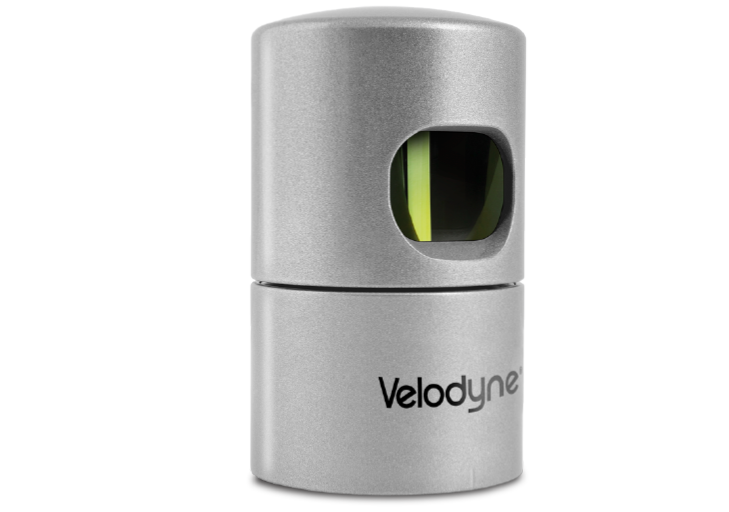
\includegraphics[scale=0.2]{velo}
    \caption{Velodyne Laser Detection and Ranging Sensor}
    \label{fig:velo}
\end{figure}
%todo bitmemis conclusion yap

\section{Localization}
In previous section, related sensors, which are used in state-of-art localization techniques, were investigated in terms of their advantages, disadvantages, and configurations. In the following sections, different localization techniques are studied under two main topics which are simultaneously localization and mapping and map-based localization.

\subsection{Simultaneously Localization and Mapping}

Simultaneous localization and mapping is a process that mobile robots build a map of the environment while they travel, and use this map concurrently to estimate its positions. This process involves so many 

\subsection{Map-Based Localization}
